\documentclass[12pt, a4paper]{article}
% pre\'ambulo
% \usepackage{helvet}
\usepackage{helvet}
\renewcommand{\familydefault}{\sfdefault}
% \usepackage{lmodern}
\usepackage[T1]{fontenc}
\usepackage[spanish,activeacute]{babel}
\usepackage{mathtools}
\usepackage{csquotes}
\usepackage{listings,lstautogobble}
\usepackage[usenames,dvipsnames]{color}
\usepackage[pdftex,bookmarksnumbered,hidelinks]{hyperref} %hyper-references%
\usepackage{float}
\usepackage{graphicx}
\graphicspath{ {images/} }


\lstset{
    language=R,
    basicstyle=\scriptsize\ttfamily,
    commentstyle=\ttfamily\color{OliveGreen},
    numbers=none,
    numberstyle=\ttfamily\color{blue}\footnotesize,
    stepnumber=1,
    numbersep=5pt,
    backgroundcolor=\color{white},
    showspaces=false,
    showstringspaces=false,
    showtabs=false,
    frame=single,
    tabsize=4,
    captionpos=b,
    breaklines=true,
    breakatwhitespace=false,
    % title=\lstname,
    escapeinside={},
    stringstyle=\ttfamily\color{OliveGreen},
    keywordstyle={\color{blue}},
    morekeywords={redundancy,TRUE, FALSE}
}

%\renewcommand{\familydefault}{\sfdefault}
\usepackage{setspace}
\spacing{1.5}

\newlength{\realoddsidemargin}	  % \oddsidemargin menos 1 in.
\newlength{\realevensidemargin}		% \evensidemargin menos 1 in.
\newlength{\realtopmargin}				% \topmargin menos 1 in.
%
% Asignaci�n de m�rgenes de p�gina
% ASIGNESE en caso de querer cambiarlo
\setlength{\realtopmargin}{2cm}			% REAL top margin.
\setlength{\realoddsidemargin}{2.5cm}		% REAL oddside margin.
\setlength{\realevensidemargin}{2.5cm}	% REAL evenside margin.
\setlength{\hoffset}{0cm}
\setlength{\voffset}{0cm}
%
% Substracci�n de 1 pulgada de compensaci�n
%  (v�ase ``Page Layout.png'' para m�s informaci�n)
\addtolength{\realoddsidemargin}{-1in}	% 1 inch = 2.54 cm.
\addtolength{\realevensidemargin}{-1in}
\addtolength{\realtopmargin}{-1in}
%
% Asignaci�n de anchuras y m�rgenes
% No hay notas al margen
\setlength{\marginparsep}{0cm} % No van a existir notas al margen
\setlength{\marginparwidth}{0cm} % No van a existir notas al margen
%
% Asignaci�n de anchura de texto
\setlength{\textwidth}{16cm}	% Anchura neta del texto (globalmente).
%
% Asignaci�n de m�rgenes par, impar y en altura
\setlength{\oddsidemargin}{\realoddsidemargin}	% odd-page left margin (global).
\setlength{\evensidemargin}{\realoddsidemargin}	% even-page left margin (global).
\setlength{\topmargin}{\realtopmargin}					% top margin (Global).



\begin{document}

\newpage
\thispagestyle{empty}
\mbox{}
\newpage
\thispagestyle{empty}
\mbox{}

\begin{titlepage}

    \begin{center}
		\normalsize {
            ESCUELA T\'ECNICA SUPERIOR DE INGENIER\'IA INFORM\'ATICA \\
            GRADO EN INGENIER\'IA INFORM\'ATICA \\
            Menci\'on en Sistemas de Informaci\'on \\}
	\end{center}

    \bigskip

    \begin{center}
		\normalsize {\textbf{
            PAQUETE R (rImplications) PARA MANIPULACI\'ON DEL CONOCIMIENTO 
            EN AN\'ALISIS FORMAL DE CONCEPTOS\\
            rImplications: Estructuras eficientes de datos para 
            implicaciones y conceptos, liber\'ias b\'asicas, 
            librer\'ias de data mining en AFC\\
            R PACKAGE (rImplications) FOR THE EFFICIENT MANIPULATION OF 
            IMPLICATIONS IN FORMAL CONCEPT ANALYSIS\\ 
            rImplications: Efficient data structures for implications 
            and concepts, basic libraries, data mining libraries in FCA
            }}
    \end{center}
    
    \smallskip

    \begin{center}
		\normalsize {
            Realizado por \\ \textbf{ANA ESPERANZA VILLAL\'ON MART\'IN}}
    \end{center}

    \begin{center}
		\normalsize {
            Tutorizado por \\ \textbf{\'ANGEL MORA BONILLA}}
    \end{center}

    \begin{center}
		\normalsize {
            Departamento \\ \textbf{MATEM\'ATICA APLICADA}}
    \end{center}

    \begin{center}
		\normalsize {
            \textbf{UNIVERSIDAD DE M\'ALAGA \\ M\'ALAGA, Julio de 2018}}
    \end{center}

    \bigskip

    \bigskip

    \begin{flushleft}
		\normalsize {
            Fecha defensa: \\ El Secretario del Tribunal}
    \end{flushleft}

\end{titlepage}

\newpage
\thispagestyle{empty}
\mbox{}

\newpage
\setcounter{page}{5}

\textbf{Resumen:} Este Trabajo Fin de Grado (TFG) tiene como objetivo principal, la creaci\'on y publicaci\'on de una librer\'ia 
en R para el An\'alisis Formal de Conceptos. Se ha realizado en la modalidad de trabajo en equipo de dos personas. 
Este trabajo se ha dividido en dos partes, teniendo partes en com\'un y partes diferenciadas en ambos. La parte conjunta 
consta de un estudio avanzado de R, as\'i como un estudio de c\'omo realizar y distribuir un paquete en R para el repositorio 
CRAN, manual de usuario y documentaci\'on del paquete completo.

La primera parte de este trabajo, se basa fundamentalmente en la creaci\'on de funciones para su posterior utilizaci\'on. Por lo que, 
en este apartado se ha desarrollado una librer\'ia b\'asica, un generador aleatorio de sistemas de implicaciones y uno de contextos, y 
por \'ultimo, una librer\'ia de funciones para el An\'alisis Formal de Conceptos, en la que se encontrar\'an las funciones m\'as importantes 
de este campo.

En la segunda parte, se podr\'a encontrar la implementaci\'on de las reglas de la L\'ogica de Simplificaciones, algoritmos desarrollados para 
el c\'alculo de cierres y eliminaci\'on de redundancias, algoritmos dedicados al c\'alculo de claves y generadores minimales y
algoritmos dedicados al c\'alculo de bases de sistemas implicacionales.

Este proyecto es una versi\'on inicial para el paquete anteriormente citado, ya que con el paso del tiempo se ir\'a mejorando y ampliando como 
el equipo del director del proyecto, es decir, \'Angel Mora, Manuel Enciso y Pablo Cordero, considere oportuno.



\bigskip

\textbf{Palabras clave:} L\'ogica de Simplificaciones, Descubrimiento de conocimiento, 
An\'alisis Formal de Conceptos, Contexto formal.

\clearpage

\textbf{Abstract:} This Degree Thesis (TFG) aims to create and publish an R package for Formal Concept Analysis. 
The TFG has been carred out by two people. The work was divided in two sections, an individual 
part and team one. The joint part has an advanced R research, a research about building and publishing 
an R package in CRAN, user manual and package documentation. 

The first part of this project is basically 
based on the creation of functions that will be used later. So, in this part, a basic library, a random 
implications system generator, a random context generator and FCA library, where the most important 
functions in this area are, have been developed. 

In the second part, we could find the Simplification 
Logic implementation, closure computing and redundancy removing algorithms, keys and minimal generators 
finding algorithms and basis computing algorithms. 

This project is an initial version of the R package 
that we mentioned before, it will be improved and extended in followings by the team of the Director of 
the project, that is, \'Angel Mora, Manuel Enciso and Pablo Cordero.

\bigskip

\textbf{Key words:} Simplification Logic,  Knowledge discovery, 
Formal Concept Analysis, Formal Context.


\newpage
\tableofcontents
\newpage
\section{Introducci\'on}

En el presente TFG se va a realizar un paquete de funciones en 
R para el \'area de An\'alisis de Conceptos formales que se ha 
constituido como una herramienta formal para el an\'alisis de datos, 
que permitir\'a la extracci\'on de conocimiento a partir de un 
conjunto de objetos y las propiedades que cumplen dichos objetos.
\\
El director del TFG (\'Angel Mora) est\'a desarrollando junto 
con su grupo de la Universidad de M\'alaga (Pablo Cordero y Manuel 
Enciso), su investigaci\'on en el \'area descrita. Actualmente, 
tienen como gran objetivo el desarrollo de una librer\'ia para el 
lenguaje R (R package) que implemente los algoritmos m\'as 
importantes que han desarrollado para la manipulaci\'on del 
conocimiento en An\'alisis de Conceptos Formales. Este TFG 
constituye la primera versi\'on del paquete que pretendemos sea 
referente para la manipulaci\'on de conocimiento en aplicaciones 
pr\'acticas.
\\
\\
Motivaci\'on:
En la actualidad, no hay una herramienta que permita el an\'alisis 
optimizado de sistemas de implicaciones en R, y aunque existen otras 
librer\'ias en otros lenguajes, no son r\'apidos o los resultados que 
muestran no llegan a ser efectivos.
Por ello, en este TFG se quiere crear un paquete de funciones que pueda 
ser difundido y usado a nivel general por cualquier persona que se dedique 
al an\'alisis de datos.
\\
\\
Objetivos:
El objetivo principal de este trabajo es obtener una librer\'ia que 
nos permita el an\'alisis r\'apido y efectivo de un conjunto de datos 
y obtener las conclusiones correctas mediante el An\'alisis de Conceptos 
Formales y sistemas de implicaciones.

Como segundo objetivo, se encuentra el de distribuir este paquete en el repositorio 
de R, para que cualquier persona interesada pueda acceder a \'el de forma sencilla.
\\
\\


\newpage
\thispagestyle{empty}
\mbox{}

\newpage

%Estructura de datos
\subsection{Estructura de datos}

Cuando se comienza a realizar un algoritmo que se necesita que 
sea r\'apido y est\'e optimizado, una de las cosas m\'as importantes 
es decidir qu\'e estructura de datos se va a utilizar.
Ya que, dependiendo de qu\'e queramos hacer, elegir bien nos puede 
ayudar a que el algoritmo se ejecute en el menor tiempo posible.

Por ello, en la gran mayor\'ia de algoritmos que se van a realizar 
en este TFG se va a utilizar la estructura rules, formada por varios 
elementos con la estructura ItemMatrix, perteneciente al paquete 
arules.
\\

La estructura de datos rules est\'a formada por cuatro slots, es decir, por 
cuatro campos de informaci\'on diferentes:

\begin{itemize}
    \item \textbf{lhs:}
    Lista de objetos de la clase ItemMatrix, en la cual se profundizar\'a m\'as 
    adelante. En este slot encontraremos todas las partes izquierdas de las 
    implicaciones, cada una de ellas con varios slots m\'as debido a que son de la 
    clase ItemMatrix. 

    \item \textbf{rhs:}
    De nuevo, es una lista de objetos de la clase ItemMatrix. S\'olo que en este 
    slot encontraremos las partes derechas de las implicaciones.

    \item \textbf{quality:}
    Objeto de la clase data.frame. En \'el se puede consultar la confianza de cada 
    una de las reglas. La confianza se define como el porcentaje de transacciones 
    que dan soporte a la regla con respecto a todas las transacciones que dan 
    soporte al cuerpo de regla. Una transacci\'on da soporte al cuerpo de regla si 
    contiene todos los items del cuerpo de regla.

    \item \textbf{info:}
    Lista con varios campos con informaci\'on del conjunto de implicaciones. Se puede 
    encontrar el nombre del dataset al que pertenecen, el n\'umero de transacciones, 
    el soporte o la confianza.

\end{itemize}


Como se ha visto en los apartados lhs y rhs, ambos est\'an formados por una lista de 
ItemMatrix, por lo que a continuaci\'on se va a detallar dicha clase, con todos sus slots.

La clase ItemMatrix es la estructura b\'asica para las transacciones, los 
conjuntos de elementos y las reglas.
La clase contiene una representaci\'on de una matriz dispersa de elementos 
y las etiquetas correspondientes a dichos elementos.

Los conjuntos de elementos se representan como matrices binarias dispersas. 
Si se trabaja con varios ItemMatrix al mismo tiempo, la codificaci\'on 
en los diferentes ItemMatrix es importante, ya que ambos elementos deben tener 
las mismas etiquetas para poder trabajar con ellos.

Cada ItemMatrix tiene la siguiente informaci\'on:
\begin{itemize}

    \item \textbf{data:}
    Objeto de la clase ngCMatrix que almacena las ocurrencias de elementos en 
    representaci\'on dispersa. Hay que tener en cuenta que ngCMatrix est\'a orientado 
    a columnas, e ItemMatrix a filas, y cada una de dichas filas representa un elemento.
    Como resultado, el ngCMatrix en este caso siempre ser\'a una versi\'on traspuesta 
    de la matriz de incidencia binaria en ItemMatrix.


    \item \textbf{itemInfo:}
    Es un data.frame que contiene vectores de longitud igual al n\'umero de elementos que 
    hay en el conjunto. Si no est\'a vac\'io, el primer elemento del data.frame debe tener 
    \textit{labels} como nombre, y contener un vector de car\'acteres con las etiquetas de los 
    elementos utilizados para representar dicho elemento. Adem\'as de estas etiquetas, el 
    data.frame puede contener vectores con nombre arbitrario, para representar, por ejemplo, 
    nombres de variables y valores que se usaron para crear los elementos binarios o 
    informaci\'on de categor\'ia jer\'arquica asociada con cada etiqueta.


    \item \textbf{itemsetInfo:}
    Es un data.frame que puede contener informaci\'on adicional para las filas en la matriz.

\end{itemize}


Veamos un ejemplo:

Si tenemos las siguientes implicaciones guardadas en la variable \textbf{rules}:
\begin{verbatim}
    a -> b
    c -> a
    d -> e
\end{verbatim}


Si ejecutamos el comando \textbf{rules@lhs@data} vamos a obtener una matriz dispersa de la clase 
ngCMatrix en la que podremos observar qu\'e elementos se encuentran en la parte izquierda de 
nuestras implicaciones.

\begin{verbatim}
    5 x 3 sparse Matrix of class "ngCMatrix"
    [1,] | . .
    [2,] . . .
    [3,] . | .
    [4,] . . |
    [5,] . . .
\end{verbatim}

Es decir, las filas son los diferentes elementos que tenemos en todas las reglas, y las 
columnas son cada una de las implicaciones.


Al ejecutar \textbf{rules@lhs@itemInfo}, vamos a obtener el nombre de cada uno de los elementos que 
tiene nuestro conjunto de implicaciones. 

\begin{verbatim}
    labels
    1      a
    2      b
    3      c
    4      d
    5      e
\end{verbatim}


Por \'ultimo, si ejecutamos \textbf{rules@lhs@itemsetInfo}, se obtiene el n\'umero de columnas y filas 
que tiene el data.frame de info. 
Como en este caso no tiene ninguna informaci\'on, obtenemos lo siguiente:
\begin{verbatim}
    data frame with 0 columns and 0 rows
\end{verbatim}


Esta estructura de datos, es bastante \'util para trabajar con conjuntos, ya que se pueden 
realizar todas las operaciones de forma eficiente, como por ejemplo, uni\'on o intersecci\'on.
Adem\'as, si se quiere obtener un conjunto de implicaciones de un dataset, al usar la funci\'on 
apriori del paquete arules, nos devolver\'a un conjunto en un ItemMatrix, por lo que nos va a 
resultar m\'as sencillo trabajar con este tipo de estructura, ya que es la m\'as 
extendida a nivel general. Por lo que a la hora de publicar el paquete de funciones, cuando otras 
personas quieran usar nuestros algoritmos, lo podr\'an realizar con facilidad, ya que se ajusta 
a c\'omo se trabaja en la actualidad en an\'alisis de datos.

As\'i que, debido a la estructura de esta clase, la facilidad de uso, y la adecuaci\'on a 
los datos que se van a utilizar a lo largo de este TFG, se ha elegido la estructura rules, compuesta de ItemMatrix 
como la principal a usar.


\clearpage

\subsection{Librer\'ia b\'asica para sistemas de implicaciones}
Se va a intentar que este paquete de funciones pueda perdurar en el tiempo, y para ello, 
se a realizado una librer\'ia b\'asica para intentar modularizar el c\'odigo y que sea lo 
m\'as legible posible a la hora de poder comprenderlo.

En esta librer\'ia b\'asica se encuentran diferentes funciones que se usar\'an bastante a lo largo de este TFG, a continuaci\'on 
se van a detallar una a una.


%%% initialize.setOfAttributes %%%
\subsubsection{Inicializar conjunto de atributos}

    \textbf{Descripci\'on}

    Esta funci\'on se utilizar\'a para inicializar un conjunto de datos, es decir, se le va a pasar un subconjunto 
    de todos los atributos que componen a un grupo de implicaciones, adem\'as del conjunto completo de los atributos. 
    
    Dentro de esta se va a utilizar la funci\'on encode para convertir el subconjunto de atributos en un objeto itemMatrix, y de esta 
    forma poder trabajar con ellos en los diferentes algoritmos que se van a desarrollar a lo largo de este TFG.

    Es decir, con esta funci\'on lo que se consigue es tener un conjunto de atributos con la estructura adecuada para poder trabajar con \'el.
    \\

    
    \textbf{C\'odigo}
    
    \lstinputlisting{r_code/basicLibrary/initialize.setOfAttributes.R}
    \bigskip
    
    \textbf{Ejemplo}

    Para que se entienda mejor esta funci\'on, se va a plantear un ejemplo:

    \begin{figure}[H]
        \centering
        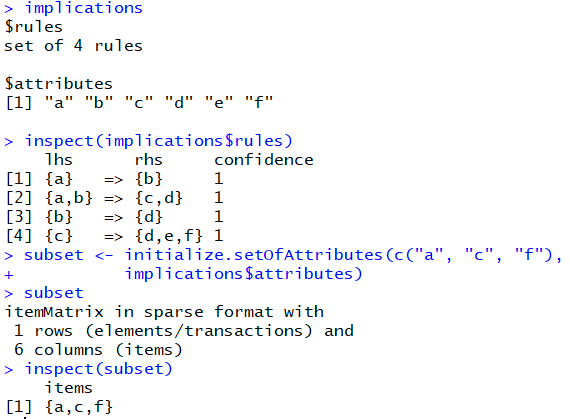
\includegraphics{InicializarConj}
        \caption{Ejemplo de inicializar conjunto de atributos}
        \label{fig:InicializarConj}
    \end{figure}

    En la variable implications se tiene un conjunto de 4 reglas y el conjunto de atributos que las componen.
    Al usar la funci\'on descrita en este punto, pas\'andole un subconjunto de todos los atributos, en este caso \{a,c,f\}, y 
    el conjunto total de los atributos, nos devuelve un itemMatrix. 
    
    Dicho itemMatrix est\'a compuesto s\'olo por esos tres atributos, aunque va a contener la informaci\'on de todos los que 
    componen las reglas; ya que deben estar para poder usar algunas funciones como uni\'on o intersecci\'on.



%%% is.singleton %%%
\subsubsection{Conjunto unitario}

    \textbf{Descripci\'on}
    
    Un conjunto unitario es aquel que tiene un s\'olo elemento. Por lo que esta funci\'on 
    devolver\'a TRUE si la longitud del conjunto que se le pase es igual a 1, o FALSE en caso 
    contrario.

    Esta es una funci\'on a la que se le puede pasar por par\'ametro una lista, un vector, 
    un conjunto de reglas o cualquier otro conjunto de elementos al que se le pueda aplicar la funci\'on 
    length().
    \\


    \textbf{C\'odigo}

    \lstinputlisting{r_code/basicLibrary/is.singleton.R}
    \bigskip

    \textbf{Ejemplo}

    En este caso, se van a proponer tres ejemplos diferentes para poder entender el comportamiento de esta funci\'on:

    \begin{figure}[H]
        \centering
        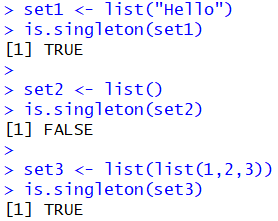
\includegraphics{singleton}
        \caption{Ejemplos de conjuntos unitarios}
        \label{fig:singleton}
    \end{figure}

    En el primer ejemplo, se puede observar que el conjunto es unitario porque est\'a compuesto por una sola cadena de caracteres. 
    Es decir, no cuenta caracter a caracter, sino la cadena, luego est\'a formado por un solo elemento y el resultado es TRUE.

    En el segundo ejemplo, tenemos una lista vac\'ia, por lo que como no tiene ning\'un elemento, el resultado es FALSE porque no es unitario.

    Por \'ultimo, se tiene una lista que contiene a otra lista con tres elementos dentro de ella. En este caso, se podr\'ia pensar que 
    no es unitario al ver los tres elementos, pero no, ya que el elemento que estamos estudiando es el primero, y este contiene solo una lista 
    en \'el, por lo que el resultado es TRUE, ya que s\'i es unitario.



%%% union.sets %%% 
\subsubsection{Uni\'on}

    \textbf{Descripci\'on}

    La uni\'on de dos conjuntos es una operaci\'on que devolver\'a otro conjunto formado por 
    todos los elementos de los dos conjuntos iniciales. Si un elemento se encuentra en los dos 
    conjuntos, s\'olo aparecer\'a una vez en el resultante.

    \[
    A \cup B = \{x\in U ~ | ~ x\in A ~ o ~ x\in B \}
    \]

    Esta funci\'on se usar\'a para la uni\'on de elementos de la clase itemMatrix, ya que lo que 
    se usa es itemUnion, una funci\'on perteneciente al paquete arules.
    \\


    \textbf{C\'odigo}

    \lstinputlisting{r_code/basicLibrary/union.sets.R}
    \clearpage

    \textbf{Ejemplo}

    \begin{figure}[H]
        \centering
        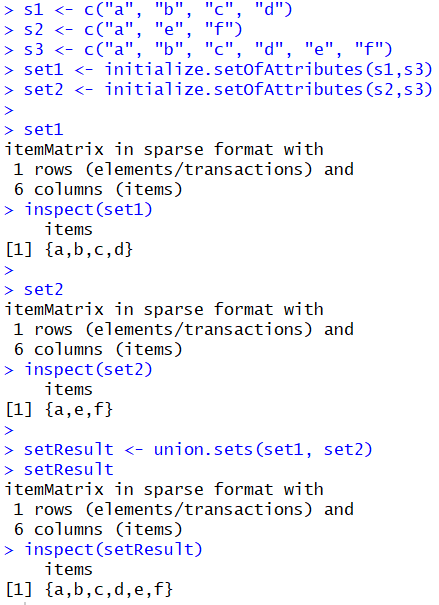
\includegraphics{union}
        \caption{Ejemplo de uni\'on de conjuntos}
        \label{fig:union}
    \end{figure}

    A continuaci\'on se va a explicar el anterior ejemplo paso a paso, ya que en \'el se han realizado varios pasos.

    Primero, se ha comenzado declarando tres vectores diferentes. Los dos primeros van a ser los dos conjuntos a unir, y el 
    tercero es la uni\'on de todas las variables. Despu\'es, se utiliza la funci\'on explicada anteriormente para convertir ambos 
    vectores en itemMatrix.

    Segundo, se observa que ambos conjuntos son de la estructura itemMatrix, con el mismo n\'umero de columnas. Esto es algo muy 
    importante, y por eso se ha usado la funci\'on initialize.setOfAttributes, ya que para utilizar la uni\'on, los elementos deben 
    estar en los dos conjuntos como informaci\'on, tal y como se vi\'o en la estructura de datos itemMatrix.

    Por \'ultimo, se realiza la uni\'on e inspeccionamos la variable resultante, y se comprueba que se ha realizado correctamente.



%%% intersection.sets %%% 
\subsubsection{Intersecci\'on}

    \textbf{Descripci\'on}
    
    La intersecci\'on de dos conjuntos A y B devolver\'a otro conjunto resultante U con los elementos 
    que se encuentren en ambos conjuntos iniciales. Es decir, el conjunto U estar\'a formado por los elementos 
    que est\'en tanto en A como en B.

    \[
        A \cap B = \{x\in U ~ | ~ x\in A ~ y ~ x\in B \}
    \]

    En este caso, tambi\'en se usar\'a con la estructura de datos itemMatrix que es la usada mayoritariamente con implicaciones 
    como ya se ha especificado antes.
    \\


    \textbf{C\'odigo}

    \lstinputlisting{r_code/basicLibrary/intersection.sets.R}
    \bigskip

    \textbf{Ejemplo}

    Para el ejemplo de esta funci\'on se van a utilizar los mismos conjuntos del ejemplo de la anterior funci\'on:

    \begin{figure}[H]
        \centering
        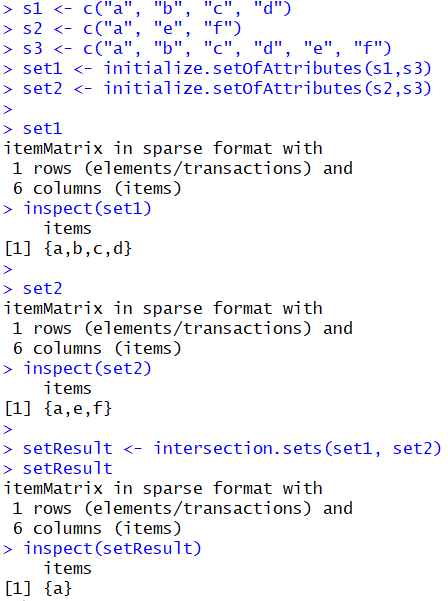
\includegraphics{interseccion}
        \caption{Ejemplo de intersecci\'on de conjuntos}
        \label{fig:interseccion}
    \end{figure}

    Para comenzar el ejemplo, se han realizado los mismos pasos que en el anterior, se declaran las variables y se convierten a 
    itemMatrix. 
    Por \'ultimo, se realiza la intersecci\'on de ambos conjuntos y vemos como el resultado es \'unicamente del elemento que se encuentra 
    en ambos conjuntos.

    \clearpage

%%% difference.sets %%% 
\subsubsection{Diferencia}

    \textbf{Descripci\'on}

    La diferencia de dos conjuntos da como resultado otro conjunto con los elementos que resultan de 
    eliminar a los elementos que forman el primer conjunto, los del segundo. Es decir, se obtendr\'ian 
    todos elementos del primer conjunto que no est\'an en el segundo.

    \[
        A - B = \{x\in A ~ y ~ x\notin B \}
    \]

    De nuevo, en nuestra funci\'on se usa una del paquete arules para poder utilizar la gran mayor\'ia de estructuras 
    que sean compatibles con restar elementos.
    \\


    \textbf{C\'odigo}

    \lstinputlisting{r_code/basicLibrary/difference.sets.R}
    \bigskip

    \textbf{Ejemplo}

    Para ilustrar bien esta funci\'on, vamos a volver a utilizar los conjuntos usados en la uni\'on e intersecci\'on para comprobar 
    cu\'al ser\'ia el resultado al realizar la diferencia de estos conjuntos.

    \begin{figure}[H]
        \centering
        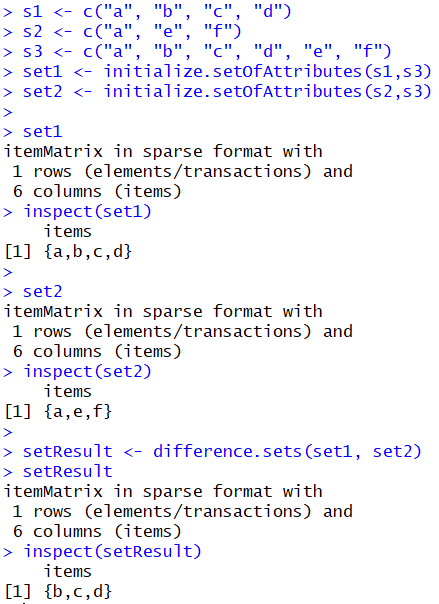
\includegraphics{diferencia}
        \caption{Ejemplo de diferencia de conjuntos}
        \label{fig:diferencia}
    \end{figure}

    En este caso, se vuelve a realizar todo de la mismo forma que en los anteriores casos, pero usamos la funci\'on difference.sets, y 
    con ella obtenemos como resultado un nuevo conjunto, en el que se encuentran los elementos del primer conjunto, eliminando los que 
    tambi\'en est\'en en el segundo.
    \clearpage


%%% is.included %%% 
\subsubsection{Inclusi\'on}

    \textbf{Descripci\'on}

    Un conjunto A est\'a incluido en un conjunto B, si A es subconjunto de B. Por lo que esta funci\'on 
    devolver\'a TRUE si cumple dicha propiedad, o FALSE en caso contrario.

    \[
        A \subseteq B ~ | ~  \forall ~ x \in A \to x \in B 
    \]

    De nuevo, esta funci\'on se utilizar\'a con elementos de la clase itemMatrix.
    \\

    \textbf{C\'odigo}

    \lstinputlisting{r_code/basicLibrary/is.included.R}
    \bigskip

    \textbf{Ejemplo}

    \begin{figure}[H]
        \centering
        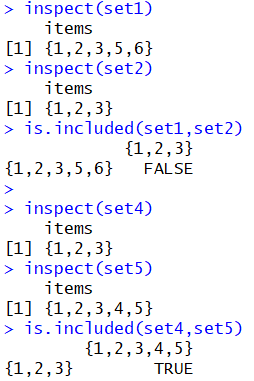
\includegraphics{inclusion}
        \caption{Ejemplos de inclusi\'on de conjuntos}
        \label{fig:inclusion}
    \end{figure}

    En este caso, se van a proponer dos ejemplos:

    En el primero no se cumple que el set1 est\'e incluido en el set2, aunque s\'i se cumplir\'ia al contrario, pero la inclusi\'on no es 
    una funci\'on que cumpla la propiedad sim\'etrica, luego en este caso el resultado es FALSE.

    En el segundo ejemplo s\'i que se cumple que el primer conjunto est\'e incluido en el segundo. Como se puede observar da igual el orden 
    en el que est\'en los elementos.



%%% is.empty.set %%% 
\subsubsection{Vac\'io}

    \textbf{Descripci\'on}

    Un conjunto es vac\'io si no contiene ning\'un elemento. Es decir, si el tama\~no del conjunto es 0, 
    podemos decir que est\'a vac\'io. 

    \[
        A = \{ \} = \emptyset
    \]

    \textbf{C\'odigo}

    \lstinputlisting{r_code/basicLibrary/is.empty.set.R}
    \bigskip

    \textbf{Ejemplo}

    \begin{figure}[H]
        \centering
        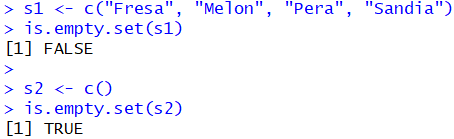
\includegraphics{vacio}
        \caption{Ejemplos de conjuntos vac\'ios}
        \label{fig:vacio}
    \end{figure}

    En el primer ejemplo, se puede ver que la funci\'on devuelve FALSE porque el conjunto contiene elementos.

    En cambio, en el segundo, el vector no contiene elementos, por lo que la funci\'on devuelve TRUE porque el conjunto no tiene 
    elementos.



    %%% equals.sets %%% 
\subsubsection{Igualdad}

    \textbf{Descripci\'on}

    Dos conjuntos A y B son iguales si su longitud es la misma, y si para cada elemento de A, existe uno igual 
    en B y para cada elemento de B existe uno igual en A.

    Ya que, seg\'un el axioma de extensionalidad:

    \[
        \forall A, B : \forall x, (x \in A \Leftrightarrow x \in B) \to A = B
    \]


    \textbf{C\'odigo}

    \lstinputlisting{r_code/basicLibrary/equals.sets.R}
    \bigskip

    \textbf{Ejemplo}

    \begin{figure}[H]
        \centering
        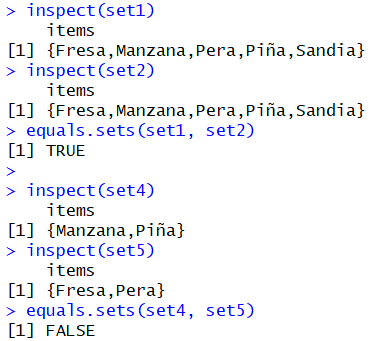
\includegraphics{igualdad}
        \caption{Ejemplos de igualdad de conjuntos}
        \label{fig:igualdad}
    \end{figure}

    De nuevo, se plantean dos ejemplos. En el primero, el resultado es TRUE, ya que visualmente se puede comprobar que ambos conjuntos son 
    iguales.

    En el segundo caso, la funci\'on devuelve FALSE porque los conjuntos no son iguales.



%%%%%%%%%%%%%%%%%%%%%%%%%%%%%%%%%%%%%%%%%%%%%%%%%%%%%%%%%%%%%%%%%%%%%%%%%%%%%%%%%%%%%%%%%%%%%%%%%%%%%%%%%%%%%%%%%%%%%%%%



%%% remove.imp %%% 
\subsubsection{Eliminar implicaci\'on}

    \textbf{Descripci\'on}

    Una de las tareas m\'as importantes de este TFG es trabajar con implicaciones. Una de las operaciones m\'as habituales 
    va a ser la de eliminar una implicaci\'on de un conjunto. Para ello, se ha definido la siguiente funci\'on, pas\'andole 
    como par\'ametros el conjunto de implicaciones y la posici\'on de la que se desea eliminar, devolver\'a un conjunto sin 
    dicha implicaci\'on.
    \\


    \textbf{C\'odigo}

    \lstinputlisting{r_code/basicLibrary/remove.imp.R}
    \bigskip

    \textbf{Ejemplo}

    \begin{figure}[H]
        \centering
        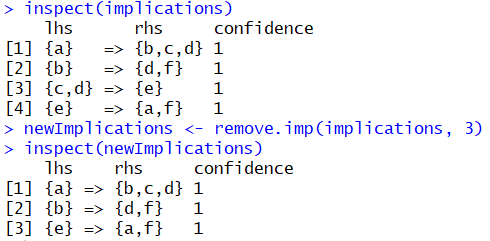
\includegraphics{removeImp}
        \caption{Ejemplo de eliminar implicaci\'on}
        \label{fig:removeImp}
    \end{figure}

    En este ejemplo, tenemos un conjunto inicial implications con cuatro implicaciones diferentes. A continuaci\'on se usa la 
    funci\'on remove.imp y con ella eliminamos la tercera.

    Finalizamos comprobando que efectivamente, en el nuevo conjunto solo se tienen tres implicaciones, quitando la tercera del conjunto 
    inicial.



%%% remove.all %%% 
\subsubsection{Vaciar conjunto}

    \textbf{Descripci\'on}

    Otra funci\'on que puede ser \'util es vaciar un conjunto. Se podr\'ia pensar que igualando el conjunto a nulo, 
    se podr\'ia obtener el resultado que se quiere conseguir. Pero no es as\'i, ya que lo que se quiere es un conjunto sin 
    elementos, pero que siga manteniendo su estructura de conjunto, no algo nulo. 
    
    Para ello, en esta funci\'on, vamos a devolver la posici\'on 0 del conjunto que se quiere vaciar. Recordemos, que en el 
    lenguaje R los arrays, listas y dem\'as estructuras de conjuntos comienzan en 1 y no en 0 como la gran mayor\'ia de lenguajes.
    Por lo que al devolver esta posici\'on, el resultado que se obtiene es el conjunto que se le hab\'ia pasado, pero sin ning\'un 
    elemento.
    \\


    \textbf{C\'odigo}

    \lstinputlisting{r_code/basicLibrary/remove.all.R}
    \bigskip

    \textbf{Ejemplo}

    \begin{figure}[H]
        \centering
        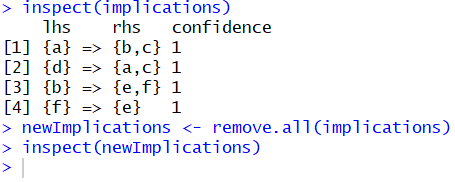
\includegraphics{removeAll}
        \caption{Ejemplo de vaciar conjunto}
        \label{fig:removeAll}
    \end{figure}

    En este caso, tenemos un conjunto de implicaciones, y si vaciamos dicho conjunto, el resultado es vac\'io ya que el nuevo 
    conjunto resultante no contiene ninguna implcaci\'on.



%%% add.imp %%% 
\subsubsection{A\~nadir implicaci\'on}

    \textbf{Descripci\'on}

    Igual que se puede querer eliminar una implicaci\'on, tambi\'en ser\'a posible a\~nadir una nueva. Por lo que esta funci\'on, 
    inserta la nueva implicaci\'on en la \'ultima posici\'on del conjunto. Como par\'ametros necesita el conjunto que se quiere ampliar, 
    el antecedente de la nueva implicaci\'on y el consecuente.

    As\'i que, se crea la nueva implicaci\'on, con las dos partes que se le pasan como par\'ametros, y se le concatena al conjunto 
    inicial para devolver un conjunto ampliado con una nueva implicaci\'on.
    \\


    \textbf{C\'odigo}

    \lstinputlisting{r_code/basicLibrary/add.imp.R}
    \bigskip

    \textbf{Ejemplo}

    \begin{figure}[H]
        \centering
        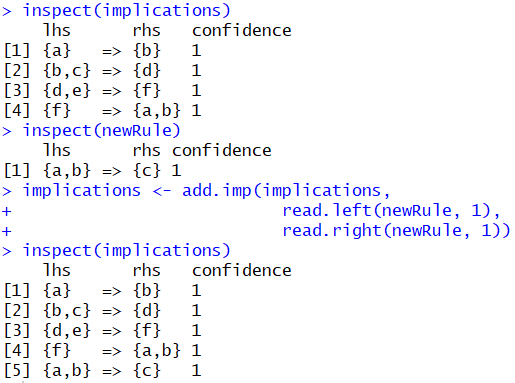
\includegraphics{addImp}
        \caption{Ejemplo de a\~nadir implicaci\'on}
        \label{fig:addImp}
    \end{figure}

    En este ejemplo tenemos un conjunto de 4 implicaciones en la variable implications, en newRule tenemos una \'unica regla que va 
    a ser la nueva a insertar. 

    Usando la funci\'on add.imp a\~nadimos la nueva regla como se puede observar en el nuevo conjunto implications.



%%% new.imp %%% 
\subsubsection{Nueva implicaci\'on}

    \textbf{Descripci\'on}

    Con esta funci\'on, vamos a insertar una nueva implicaci\'on, al igual que en el punto anterior, pero esta vez 
    de una forma un poco m\'as compleja. Ya que, en este caso, se van a realizar varias comprobaciones.

    Para cada implicaci\'on perteneciente al conjunto, se va a comprobar si el antecedente es igual al que se quiere insertar.
    En caso negativo, se continuar\'a con la siguiente implicaci\'on; y en caso afirmativo, se comprobar\'a si los consecuentes son 
    iguales. En caso de que se cumplan ambas afirmaciones, quiere decir que la implicaci\'on que intentamos insertar en el conjunto, 
    ya se encuentra en \'el, por lo que se devolver\'a el conjunto inicial sin ning\'un cambio.

    En el caso de que los antecedentes sean iguales, y los consecuentes no, se sustituir\'a esa regla por una nueva, en la que el antecedente 
    queda igual, y el consecuente estar\'a formado por la uni\'on del que ya estaba en el conjunto, y el nuevo que se quiere insertar. Y con 
    esto, se devolver\'ia el nuevo conjunto.

    El \'ultimo caso que se podr\'ia dar, es aquel en el que ninguna implicaci\'on del conjunto tenga el mismo antecedente que el que se 
    quiere insertar, por lo que al finalizar la iteraci\'on por todo el conjunto, se insertar\'ia la nueva regla y devolver\'ia el conjunto 
    resultante.
    \\

    \clearpage

    \textbf{C\'odigo}

    \lstinputlisting{r_code/basicLibrary/new.imp.R}
    \bigskip

    \textbf{Ejemplo}


    \begin{figure}[H]
        \centering
        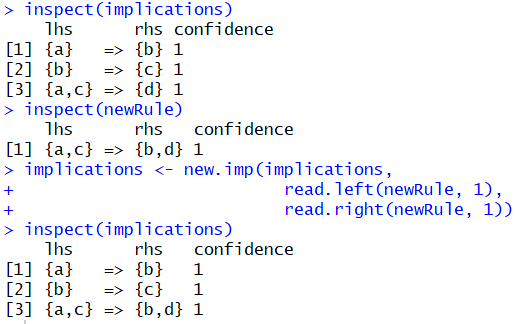
\includegraphics{newImp}
        \caption{Ejemplo de a\~nadir implicaci\'on}
        \label{fig:newImp}
    \end{figure}

    Aunque con esta funci\'on se podr\'ian realizar varios ejemplos seg\'un la implicaci\'on que se quiera a\~nadir, en este caso se 
    va a insertar una nueva en la que el antecedente ya se encuentra en el conjunto y el consecuente es nuevo.

    En la variable implications tenemos un conjunto de tres implicaciones, y en newRule, est\'a la nueva a insertar. Como se puede 
    observar, el antecedente de la nueva es igual al de la tercera implicaci\'on del conjunto. Se realiza la operaci\'on de a\~nadir 
    y vemos como en el conjunto resultante ha cambiado el consecuente de la \'ultima implicaci\'on tal y como se esperaba.



%%% read.left %%% 
\subsubsection{Leer antecedente}

    \textbf{Descripci\'on}

    Otra de las funciones b\'asicas a la hora de trabajar con implicaciones es poder obtener el antecedente de una determinada 
    implicaci\'on. Para ello, pas\'andole a esta funci\'on el conjunto que contiene a la implicaci\'on que queremos obtener, y su 
    posici\'on, nos devolver\'a el antecedente deseado.
    \\


    \textbf{C\'odigo}

    \lstinputlisting{r_code/basicLibrary/read.left.R}
    \bigskip

    \textbf{Ejemplo}

    Aunque esta funci\'on ya se ha utilizado en algunos ejemplos anteriores, veamos su resultado.

    \begin{figure}[H]
        \centering
        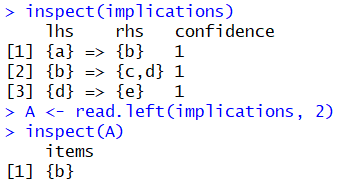
\includegraphics{readL}
        \caption{Ejemplo de leer antecedente}
        \label{fig:readL}
    \end{figure}

    Luego, en este ejemplo, tenemos un conjunto de tres implicaciones y con esta funci\'on leemos, en este caso, el antecedente de 
    la segunda implicaci\'on. 



%%% read.right %%% 
\subsubsection{Leer consecuente}

    \textbf{Descripci\'on}
    
    De igual forma que en el anterior punto, se puede querer obtener el consecuente de una implicaci\'on, luego, con el conjunto de 
    implicaciones y su posici\'on, esta funci\'on devolver\'a el consecuente de dicha implicaci\'on.
    \\


    \textbf{C\'odigo}

    \lstinputlisting{r_code/basicLibrary/read.right.R}
    \bigskip

    \textbf{Ejemplo}

    Al igual que en el anterior punto, esta funci\'on ya se ha usado en ejemplos anteriores, pero observemos cual es su resultado.

    \begin{figure}[H]
        \centering
        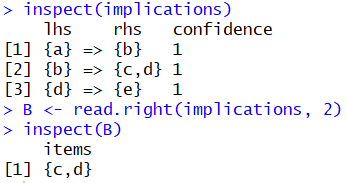
\includegraphics{readR}
        \caption{Ejemplo de leer consecuente}
        \label{fig:readR}
    \end{figure}

    Para este ejemplo, se ha usado el mismo conjunto de implicaciones que en el anterior, y leemos el consecuente de la misma 
    implicaci\'on que en el punto anterior.

    \clearpage

%%% substitute.imp %%% 
\subsubsection{Sustituir implicaci\'on}

    \textbf{Descripci\'on}

    La sustituci\'on de una implicaci\'on es una operaci\'on bastante \'util, ya que cuando se quieren unir dos implicaciones, puede que 
    se quiera que la nueva permanezca en un lugar determinado, para ello, esta funci\'on inserta la nueva implicaci\'on en el lugar que 
    se le indique. Como par\'ametros, necesita el conjunto de implicaciones, la posici\'on a cambiar, y los nuevos antedecente y consecuente.
    Para la utilizaci\'on de esta funci\'on se debe llamar a sustitute.imp, aunque esta, a su vez har\'a uso de add.imp.k, cuyos codigos se 
    muestran a continuaci\'on. 
    \\


    \textbf{C\'odigo}

    \lstinputlisting{r_code/basicLibrary/add.imp.k.R}

    \lstinputlisting{r_code/basicLibrary/substitute.imp.R}
    \bigskip

    \textbf{Ejemplo}

    \begin{figure}[H]
        \centering
        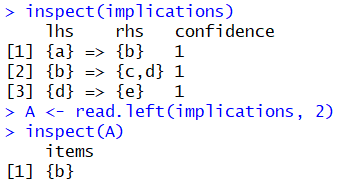
\includegraphics{readL}
        \caption{Ejemplo de leer antecedente}
        \label{fig:readL}
    \end{figure}

    Comenzamos con un conjunto de tres implicaciones en la variable implications, en newRule se tiene la implicaci\'on que se va 
    a insertar en el conjunto. Realizamos la operaci\'on de sustituir, en este caso la segunda implicaci\'on del conjunto, por la nueva. 
    Tal y como se observa en el conjunto resultante, se ha sustituido la anterior, por la nueva, tal y como se esperaba.


%%% included.left %%% 
\subsubsection{Incluido en antecedente}

    \textbf{Descripci\'on}

    Si tenemos dos implicaciones A y B y se quiere comprobar si el antecedente de A est\'a incluido en el de B, se debe usar 
    esta funci\'on. Le pasamos como par\'ametros un conjunto de implicaciones, y dos posiciones de dicho conjunto. Se usar\'an 
    las funciones is.included y read.left para comprobar si un antecedente est\'a incluido en otro, devolver\'a TRUE en caso 
    afirmativo, y FALSE en el contrario.
    \\


    \textbf{C\'odigo}

    \lstinputlisting{r_code/basicLibrary/included.left.R}
    \bigskip

    \textbf{Ejemplo}

    \begin{figure}[H]
        \centering
        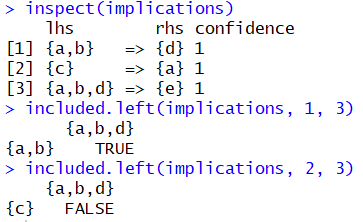
\includegraphics{incluidoL}
        \caption{Ejemplo de leer antecedente}
        \label{fig:incluidoL}
    \end{figure}

    Para este ejemplo tenemos un conjunto con tres implicaciones. Primero se comprueba si el antecedente de la primera implicaci\'on 
    est\'a incluido en el de la segunda, el resultado obtenido es TRUE, ya que se cumple la inclusi\'on.

    En cambio, en el segundo caso, se prueba el consecuente de la segunda, con el de la tercera, y como no se cumple, el resultado es FALSE.



%%% delete.set.of.IS %%% 
\subsubsection{Eliminar implicaciones con consecuente vac\'io}

    \textbf{Descripci\'on}

    Si se tiene un conjunto de implicaciones y alguna de ellas tiene su consecuente vac\'io, esta implicaci\'on no va a 
    aportar ning\'un tipo de conocimiento a este conjunto, por lo que se deben eliminar. Para ello, se usar\'ia esta funci\'on, 
    la cual, pas\'andole como par\'ametro dicho conjunto, nos devolver\'a uno nuevo eliminando las implicaciones con su consecuente 
    vac\'io.
    \\


    \textbf{C\'odigo}

    \lstinputlisting{r_code/basicLibrary/delete.set.of.IS.R}
    \bigskip

    \textbf{Ejemplo}

    \begin{figure}[H]
        \centering
        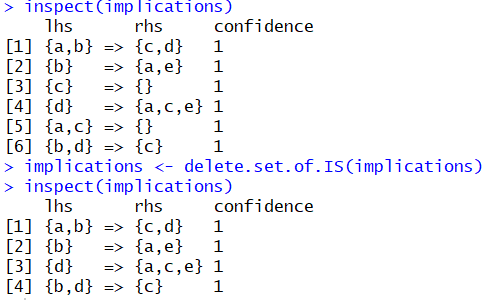
\includegraphics{deleteIS}
        \caption{Ejemplo de eliminar implicaciones con consecuente vac\'io}
        \label{fig:deleteIS}
    \end{figure}

    Comenzamos con un conjunto de seis implicaciones, en el que dos de ellas tienen su consecuente vac\'io. Al realizar la 
    operaci\'on de borrar los consecuentes vacios, obtenemos un nuevo conjunto con cuatro implicaciones, ya que las que ten\'ian 
    sus consecuentes sin elementos, han sido eliminadas.



%%% size.set %%% 
\subsubsection{Tama\~no del conjunto}

    \textbf{Descripci\'on}

    Por tama\~no del conjunto, se entiende el n\'umero de elementos, repetidos o no, que lo componen. 
    Es decir, para calcular el tama\~no de un conjunto, se va a realizar la suma de los tama\~nos de cada una de 
    las implicaciones que forman el conjunto.
    \\


    \textbf{C\'odigo}

    \lstinputlisting{r_code/basicLibrary/size.set.R}
    \bigskip

    \textbf{Ejemplo}

    \begin{figure}[H]
        \centering
        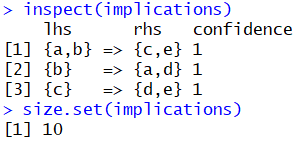
\includegraphics{size}
        \caption{Ejemplo de tama\~no de conjunto}
        \label{fig:size}
    \end{figure}

    En este ejemplo se tiene un conjunto con tres implicaciones, su tama\~no, tal y como muestra el ejemplo es de 10. 
    Este resultado viene de sumar cu\'antos elementos tiene cada implicaci\'on, en este caso:
    \[
        4 + 3 + 3 = 10    
    \]



%%% cadinality.set %%% 
\subsubsection{Cardinalidad del conjunto}

    \textbf{Descripci\'on}

    La cardinalidad de un conjunto, se entiende como el n\'umero de implicaciones que lo componen. Es decir, lo que 
    tambi\'en se suele denominar como longitud del conjunto.
    \\


    \textbf{C\'odigo}

    \lstinputlisting{r_code/basicLibrary/cardinality.set.R}
    \bigskip

    \textbf{Ejemplo}


    \begin{figure}[H]
        \centering
        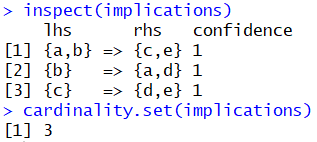
\includegraphics{cardinality}
        \caption{Ejemplo de cardinalidad de conjunto}
        \label{fig:cardinality}
    \end{figure}

    La cardinalidad, tal y como se ha explicado arriba es el n\'umero de implicaciones que tiene un conjunto, por lo que como 
    se puede observar en este ejemplo, como tiene tres implicaciones, su cardinalidad es tres.



%%% core %%% 
\subsubsection{Core}

    \textbf{Descripci\'on}

    A esta funci\'on se le pasa un conjunto de atributos Omega, junto con un conjunto de implicaciones Gamma. 
    Devolver\'a un conjunto de datos resultante de eliminar de Omega todos los atributos que se encuentren en los 
    consecuentes de las implicaciones que forman Gamma. 

    \[
        core(\Omega , \Gamma ) = \Omega ~ \textbackslash ~ ( \bigcup_{A \to B \in \Gamma} B )    
    \]
    
    Esta no es precisamente una funci\'on b\'asica, pero se ha incluido en este apartado, ya que se utilizar\'a 
    en el algoritmo de claves minimales realizado en el segundo tomo de este TFG.
    \\


    \textbf{C\'odigo}

    \lstinputlisting{r_code/basicLibrary/core.R}
    \bigskip

    \textbf{Ejemplo}


    \begin{figure}[H]
        \centering
        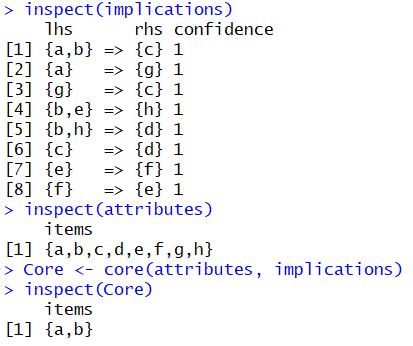
\includegraphics{core}
        \caption{Ejemplo de core de un conjunto}
        \label{fig:core}
    \end{figure}

    En el ejemplo, tenemos como punto de partida un conjunto con cinco implicaciones y todos los elementos de ese conjunto en 
    un itemMatrix. Realizamos la operaci\'on core y se obtiene como resultado un itemMatrix con dos de los elementos de las implicaciones. 
    Tal y como se ha explicado anteriormente, este resultado se obtiene de restar de todos los atributos, los que est\'an en los consecuentes 
    de las implicaciones.



%%% body %%% 
\subsubsection{Body}

    \textbf{Descripci\'on}

    Al igual que en el punto anterior, esta funci\'on se utilizar\'a en el algoritmo para calcular claves minimales, aunque junto con 
    el anterior, se han incluido aqu\'i.

    Siendo Omega un conjunto de atributos, y Gamma un conjunto de implicaciones, se define la funci\'on body como la diferencia 
    de la uni\'on de los antecedentes de Gamma, menos el cierre del core de Omega y Gamma. 

    \[
        body(\Omega , \Gamma ) = ( \bigcup_{A \to B \in \Gamma} B ) ~ \textbackslash ~ core(\Omega , \Gamma )^+
    \]

    \textbf{C\'odigo}

    \lstinputlisting{r_code/basicLibrary/body.R}
    \clearpage

    \textbf{Ejemplo}


    \begin{figure}[H]
        \centering
        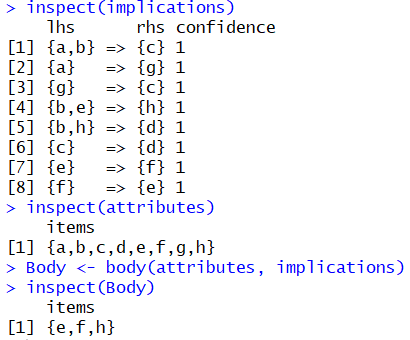
\includegraphics{body}
        \caption{Ejemplo de body de un conjunto}
        \label{fig:body}
    \end{figure}

    Para este ejemplo, se usa el mismo conjunto de implicaciones que en el anterior punto. Sin embargo, el resultado en este caso es 
    el conjunto vac\'io, ya que es el resultado de restar de todos los elementos que se encuentran en los antecedentes de las implicaciones, 
    el resultado de el cierre del core de Omega y Gamma.

    
\clearpage

\section{Generadores aleatorios}

\subsection{Sistemas de implicaciones aleatorios}

    \textbf{Introducci\'on}

    Cuando se quieren realizar pruebas con un algoritmo, se aconseja utilizar conjuntos generados de forma aleatoria, para que, por ejemplo, 
    en los an\'alisis de tiempo, los resultados no sean influidos por dichos conjuntos. Actualmente, hasta donde se conoce, no existe un 
    generador aleatorio de sistemas de implicaciones en ninguna de las diferentes \'areas, como pueden ser data mining, machine learning, 
    IA, sistemas inteligentes, redes neuronales...

    Luego, debido a esto, se ha decidido realizar una funci\'on que pueda ser usada para este fin y ponerla a disposici\'on de toda la comunidad 
    junto a este paquete.
    \\ 


    \textbf{Descripci\'on}
    
    Esta funci\'on va a generar uno o m\'as sistemas de implicaciones siguiendo una serie de par\'ametros que se pueden elegir a la 
    hora de ejecutar dicha funci\'on para obtener el conjunto como sea m\'as adecuado a lo que se desee hacer.

    Los atributos de las implicaciones van a ser del tipo a0, a1... Comenzando en 0, de forma consecutiva hasta el n\'umero que sea 
    necesario para tener todos los atributos que el usuario quiera. Los par\'ametros de esta funci\'on son:

    \begin{itemize}
        \item \textbf{numAttributes:}

        Aqu\'i se debe especificar cu\'antos atributos diferentes se quiere que tengan las implicaciones que se van a generar. Es un 
        par\'ametro obligatorio para la utilizaci\'on de esta funci\'on. Como se ha comentado anteriormente, los atributos ser\'an de la 
        forma a0, a1, a2... El valor de este par\'ametro debe ser mayor que 0.

        \clearpage

        \item \textbf{numDependencies:}

        Otro par\'ametro obligatorio es el n\'umero de dependencias que se quieren obtener, si se elige obtener m\'as de un archivo 
        con diferentes sistemas de implicaciones, como se ver\'a m\'as adelante, cada uno de dichos ficheros incluir\'a el n\'umero 
        de implicaciones que se le indique aqu\'i. Por supuesto, el valor de este par\'ametro tambi\'en debe ser mayor que 0.

        
        \item \textbf{difference:}

        Este par\'ametro opcional indica el n\'umero m\'aximo de diferencia de elementos entre el antecedente y el consecuente. Se puede 
        insertar un n\'umero negativo, lo que indicar\'a que se desea que haya m\'as atributos en el consecuente. Por lo que, si el n\'umero 
        es positivo, el antecedente tendr\'a m\'as atributos.

        En este caso, hay que tener en cuenta que el valor absoluto del n\'umero insertado en este par\'ametro, debe ser menor 
        que el n\'umero total de atributos.

        En caso de no especificar nada, la diferencia de atributos entre antecedente y consecuente ser\'a aleatoria.


        \item \textbf{percentage:}

        Este par\'ametro es bastante parecido al anterior, solo que en este caso, se trata del m\'aximo porcentaje de diferencia entre 
        el antecedente y el consecuente. Al igual que en el anterior, si el porcentaje es negativo, el consecuente ser\'a mayor, y en caso de 
        ser positivo, el antecedente tendr\'a m\'as atributos que el consecuente. Al ser un porcentaje, el valor debe ser menor estricto que 
        100.

        Cabe especificar, que tanto este par\'ametro, como el anterior, se tratan de tama\~nos m\'aximos, es decir, que no todas las implicaciones 
        van a tener la diferencia exacta que se le especifique entre antecedente y consecuente, sino que el n\'umero o porcentaje ser\'a la 
        mayor diferencia que se encontrar\'a en el sistema de implicaciones.


        \item \textbf{maxLeftSize:}

        Con este par\'ametro opcional, se puede especificar el n\'umero de elementos m\'aximo que se quiere que tenga el antecedente, como 
        es de esperar, no debe superar al n\'umero total de atributos.


        \item \textbf{maxRightSize:}

        Junto con el anterior, podemos especificar, en este caso, el n\'umero de elementos m\'aximo del consecuente. Ambos son par\'ametros 
        opcionales, pero si el usuario decide especificar el tama\~no m\'aximo del antecedente, tambi\'en deber\'a hacer lo mismo con el 
        consecuente y viceversa.


        \item \textbf{nameExitFile:}

        Este se trata de un par\'ametro obligatorio, se le debe pasar una cadena de caracteres sin la extensi\'on del archivo, ya que 
        la funci\'on devolver\'a un archivo con extensi\'on .R.


        \item \textbf{numFiles:}

        Por \'ultimo, un par\'ametro opcional en el que se puede especificar cu\'antos ficheros se quiere que se generen. Si no se especifica, 
        solo se generar\'a un archivo, en caso contrario, los archivos tendr\'an como nombre el especificado seguido de un guion bajo y un n\'umero 
        para distinguirlos.

    \end{itemize}

    Hay que precisar, que algunos de los par\'ametros anteriores son excluyentes. Es decir, si se especifica el par\'ametro difference, tanto 
    percentage, como maxLeftSize y maxRightSize deben dejarse nulos. O si se especifica percentage, deber\'an quedar vac\'ios difference y 
    maxLeftSize y maxRightSize. 
    En cambio, maxLeftSize siempre debe ir acompa\~nado de maxRightSize y viceversa, aunque en caso de especificarlos, difference y percentage, 
    deben estar nulos.
    Los par\'ametros que siempre se le deben pasar a la funci\'on son: numAttributes, numDependencies y nameExitFile.

    Por \'ultimo, hay que especificar que el sistema o sistemas de implicaciones que se obtengan, no tendr\'an redundancias y se habr\'a aplicado 
    la funci\'on de composici\'on, por lo que al realizar todas estas operaciones, si el n\'umero de implicaciones que se quiere obtener es 
    alto, el tiempo que tardar\'a el algoritmo en obtener dicho sistema, tambi\'en ser\'a alto.
    \\

    \bigskip

    \textbf{C\'odigo}

    \lstinputlisting{r_code/randomGenerators/randomImp.R}
    \clearpage


    \textbf{Ejemplo}

    Como se ha visto anteriormente, este algoritmo se puede utilizar con muchas combinaciones diferentes dependiendo de los par\'ametros 
    que se utilicen. As\'i que, se van a proponer tres ejemplos diferentes de c\'omo usar esta funci\'on, aunque las posibilidades 
    son mucho mayores.

    \bigskip

    \begin{figure}[H]
        \centering
        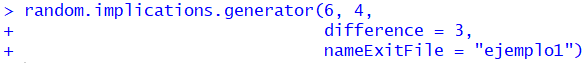
\includegraphics{randomImp1}
        \caption{Ejemplo 1 de sistemas de implicaciones aleatorios}
        \label{fig:randomImp1}
    \end{figure}

    En este primer ejemplo, se va a generar un sistema con cuatro implicaciones, utilizando 6 atributos diferentes, con una diferencia m\'axima 
    de 3 elementos entre el antecedente y el consecuente, siendo mayor el antecedente, como nombre del fichero se utilizar\'a ejemplo1.
    
    En dicho fichero se ha escrito lo siguiente:

    \begin{verbatim}
        a1 a3 a4 a6 -> a5 
        a1 a2 a4 a5 -> a6 
        a3 a6 -> a4 
        a1 a2 a6 -> a3    
    \end{verbatim}


    \begin{figure}[H]
        \centering
        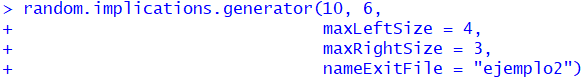
\includegraphics{randomImp2}
        \caption{Ejemplo 2 de sistemas de implicaciones aleatorios}
        \label{fig:randomImp2}
    \end{figure}

    En este segundo ejemplo se han generado con 10 atributos, 6 implicaciones, con un tama\~no m\'aximo de 4 para el antecedente y 3 para el 
    consecuente. El nombre del fichero de salida ser\'a ejemplo2.

    \begin{verbatim}
        a1 a10 a6 a7 -> a9 
        a5 -> a4 
        a10 a3 a6 a8 -> a9 
        a8 -> a9 
        a1 a10 a6 -> a7 
        a3 a7 a9 -> a4 
    \end{verbatim}
    Como se puede observar, la salida cumple todos los requisitos que le hemos puesto. En este caso, se observa que solo se han usado 9 de 
    los 10 atributos que se ped\'ian, ya que con la simplificaci\'on del conjunto, se ha llegado a perder el atributo a2.
    \\
    
    \bigskip

    Por \'ultimo, se ejecuta una tercera vez esta funci\'on para comprobar c\'omo es el error que se produce, en este caso, al pasarle vac\'io 
    el nombre del fichero de salida:

    \begin{figure}[H]
        \centering
        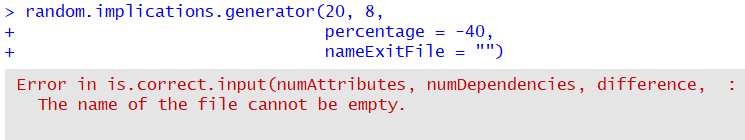
\includegraphics{randomImp3}
        \caption{Ejemplo 3 de sistemas de implicaciones aleatorios}
        \label{fig:randomImp3}
    \end{figure}

    \clearpage


\subsection{Contextos aleatorios}

    \textbf{Introducci\'on}

    En este caso, al igual que en el anterior, hasta donde se sabe, en la comunidad de FCA tampoco existe ning\'un generador aleatorio de 
    contextos, y son bastante necesarios para, como se ha nombrado antes, por ejemplo, realizar pruebas de los diferentes algoritmos.

    As\'i que, se decide realizar un algoritmo de este tipo para a\~nadirlo a este paquete para que toda persona interesada pueda 
    utilizarlo.
    

    \textbf{Descripci\'on}

    Un contexto formal \( (G, M, I) \) consiste en dos conjuntos, G y M, y una relaci\'on binaria \( I \subseteq G x M \). Los elementos 
    de G se llaman objetos, los de M, atributos de \( (G, M, I) \). Si \(g \in G ~ y ~ m \in M \) est\'an relacionados seg\'un I, se escribir\'a 
    \( (g,m) \in I ~ o ~ g I m \) y se leer\'a como ``el objeto g tiene el atributo m".

    \textcolor{red}{A\~nadir referencia paper}

    La manera habitual de representar un contexto formal es mediante una tabla, la cual contar\'a con una fila para cada objeto y una columna 
    para cada atributo, con una cruz en la intersecci\'on entre una fila g con una columna m sii el objeto g tiene un atributo m, \( (g,m) \in 
    I \).

    Por ello, la estructura m\'as sencilla a la hora de programar un algoritmo para contextos formales en R ser\'a un data.frame.
    \\


    Luego, en este caso, esta funci\'on va a generar un contexto formal siguiendo algunos par\'ametros que se pueden elegir a la 
    hora de ejecutar dicha funci\'on para obtener el contexto lo m\'as adecuado posible para lo que se desee.

    Los objetos del contexto se van a representar como obj1, obj2... y los atributos como att1, att2... Ambos comenzando en 1, de forma 
    consecutiva hasta el n\'umero que el usuario indique.
    \\

    Los par\'ametros de esta funci\'on son:

    \begin{itemize}
        \item \textbf{num.obj:}

        Con este par\'ametro obligatorio se indicar\'a el n\'umero de objetos que debe tener el contexto, o lo que es lo mismo, 
        cu\'antas filas tendr\'a el data.frame. Este par\'ametro debe ser mayor que uno, 
        ya que no tendr\'ia sentido crear un contexto sin objetos.


        \item \textbf{num.attr:}

        Este par\'ametro obligatorio indicar\'a cual ser\'a el n\'umero de atributos del contexto, es decir, las columnas que tendr\'a el 
        data.frame. De nuevo, debe ser un n\'umero mayor que uno, ya que tampoco tendr\'ia sentido en este caso crear un contexto sin 
        atributos.

        \item \textbf{sparness:}

        Como par\'ametro opcional, tenemos la dispersi\'on, es decir la probabilidad de que un objeto tenga un atributo, o lo que es 
        lo mismo a la hora de programarlo, que en el cruce de columna y fila, haya un uno.
        Como este par\'ametro se trata de una probabilidad, su valor debe estar entre 0 y 1.

    \end{itemize}


    Cuando se utilice la funci\'on, esta devolver\'a un data.frame, siendo los nombres de filas los objetos, y los de las columnas 
    los atributos.


    \bigskip

    \textbf{C\'odigo}

    A la hora de optimizar el c\'odigo, si el par\'ametro sparness no est\'a vac\'io, se ha decidido generar aleatoriamente el n\'umero de 
    TRUE o FALSE dependiendo de cu\'al de los dos sea menor. Es decir, si el usuario inserta en el par\'ametro sparness 0.2, con 4 objetos 
    y 5 atributos, esto querr\'a decir que debe haber cuatro TRUE entre los 20 elementos a generar aleatoriamente. Por lo que en este caso, 
    el n\'umero de TRUE ser\'a menor que el de FALSE, as\'i que se colocar\'an cuatro TRUE aleatoriamente, rellenando las dem\'as posiciones 
    del data.frame de FALSE.

    Como el algoritmo se va a ejecutar de formas diferentes dependiendo de las entradas que elija el usuario, se ha decidido modularizarlo 
    para poder comprenderlo bien. Veamos las diferentes partes:


    Aqu\'i tenemos el algoritmo principal, que ser\'a el que el usuario utilice:

    \lstinputlisting{r_code/randomGenerators/context.R}
    \bigskip

    En el caso de que el usuario no especifique el par\'ametro sparness, el contexto se generar\'a totalmente de forma aleatoria:

    \lstinputlisting{r_code/randomGenerators/noSpar.R}
    \clearpage

    Y como se ha especificado anteriormente, dependiendo de cu\'al sea la probabilidad de dispersi\'on elegida por el usuario, se generar\'an 
    los TRUE o los FALSE:

    \lstinputlisting{r_code/randomGenerators/ones.R}
    \bigskip
    \lstinputlisting{r_code/randomGenerators/zeros.R}
    \bigskip

    \textbf{Ejemplo}

    Como primer ejemplo, se va a generar un contexto sin el par\'ametro sparness, con 4 objetos y 5 atributos:

    \begin{figure}[H]
        \centering
        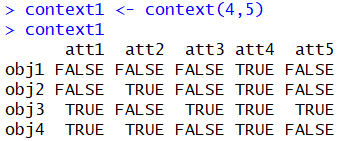
\includegraphics{randomC1}
        \caption{Ejemplo 1 de contextos aleatorios}
        \label{fig:randomC1}
    \end{figure}

    \bigskip
    Y como segundo ejemplo, un contexto con 6 objetos y 8 atributos, con 0.5 de sparness:

    \begin{figure}[H]
        \centering
        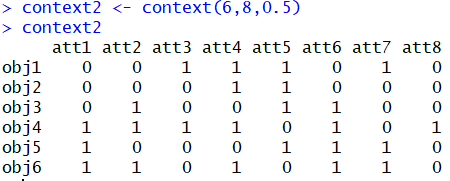
\includegraphics{randomC2}
        \caption{Ejemplo 2 de contextos aleatorios}
        \label{fig:randomC2}
    \end{figure}

    Como podemos observar, el n\'umero de FALSE y TRUE es el mismo, ya que se ha elegido como par\'ametro de esparness 0.5.
    
\clearpage

\subsection{Librer\'ia de An\'alis de Conceptos Formales}

\textbf{Introducci\'on}

El ana\'alis de conceptos formales es un entorno conceptual que estructura, analiza y visualiza conocimiento a partir de datos proporcionados 
como una relaci\'on binaria entre objetos y atributos.

Como se ha explicado anteriormente, un contexto formal \( (G, M, I) \) consiste en dos conjuntos, G y M, y una relaci\'on binaria \( I \subseteq G x M \). Los elementos 
de G se llaman objetos, los de M, atributos de \( (G, M, I) \). Si \(g \in G ~ y ~ m \in M \) son una relaci\'on I, se escribir\'a 
\( (g,m) \in I ~ o ~ g I m \) y se leer\'a como ``el objeto g tiene el atributo m".

Para trabajar con contextos se utilizan varias funciones que se van a desgranar una a una en los siguientes puntos:

    \subsubsection{Leer concepto}

        \textbf{Descripci\'on}

        Como primera funci\'on se tiene la de obtener un concepto formal con su estructura adecuada teniendo la informaci\'on en un fichero. A la 
        hora de utilizar esta funci\'on se pueden usar ficheros xls, txt o r, ya que el resultado ser\'a el mismo, una variable de tipo data.frame 
        con toda la informaci\'on del fichero de entrada.

        \textbf{C\'odigo}

        \lstinputlisting{r_code/FCA/read.fc.R}

        \textbf{Ejemplo}



    %Mp y mp2
    \subsubsection{Operador de derivaci\'on de atributos a objetos}

        \textbf{Descripci\'on}

        Dado un contexto formal \( (G, M, I) \), se llama operador de derivaci\'on de atributos a objetos a la 
        funci\'on \( ^\uparrow : 2^G \rightarrow 2^M \)

        \( ^\uparrow = { m \in M | <g,m> \in I ~ para ~ todo ~ g \in A } \)

        El conjunto \( A^\uparrow \) es el de los atributos compartidos por todos los objetos de A, es decir, este operador devolver\'a 
        un conjunto de attributos que ser\'an los que contiene un determinado objeto.


        \textbf{C\'odigo}

        \lstinputlisting{r_code/FCA/mp.R}


        \textbf{Ejemplo}


    \subsubsection{Operador de doble derivaci\'on de atributos a objetos}

        \textbf{Descripci\'on}

        El conjunto que devuelve el operador \( A^\uparrow \) tambi\'en se suele representar como \( A' \), por lo que en este caso, 
        el operador de doble derivaci\'on de atributos a objetos se representar\'a como \( A'' \).


        \( A'' = (A^\uparrow)^\downarrow \)

        Es decir, al conjunto que se obtiene como salida del operador de derivaci\'on de atributos a objetos, se le aplica el operador 
        de derivaci\'on de objetos a atributos.


        \textbf{C\'odigo}

        \lstinputlisting{r_code/FCA/mp2.R}


        \textbf{Ejemplo}


    %Gp y Gp2
    \subsubsection{Operador de derivaci\'on de objetos a atributos}

        \textbf{Descripci\'on}

        Dado un contexto formal \( (G, M, I) \), se llama operador de derivaci\'on de objetos a atributos a la 
        funci\'on \( ^\downarrow : 2^M \rightarrow 2^G \)

        \( ^\downarrow = { g \in G | <g,m> \in I ~ para ~ todo ~ m \in B } \)

        El conjunto \( B^\downarrow \) es el de los objetos compartidos por todos los atributos de B, en este caso, este operador devolver\'a 
        un conjunto de objetos que ser\'an los que contiene un determinado atributo.

        \textbf{C\'odigo}

        \lstinputlisting{r_code/FCA/gp.R}

        \textbf{Ejemplo}


    \subsubsection{Operador de doble derivaci\'on de objetos a atributos}

        \textbf{Descripci\'on}

        El conjunto que devuelve el operador \( B^\downarrow \) tambi\'en se suele representar como \( B' \), por lo que en este caso, 
        el operador de doble derivaci\'on de objetos a atributos se representar\'a como \( B'' \).


        \( B'' = (B^\downarrow)^\uparrow \)

        Es decir, al conjunto que se obtiene como salida del operador de derivaci\'on de objetos a atributos, se le aplica el operador 
        de derivaci\'on de atributos a objetos.


        \textbf{C\'odigo}

        \lstinputlisting{r_code/FCA/gp2.R}


        \textbf{Ejemplo}



    \subsubsection{Crear contexto}

        \textbf{Descripci\'on}

        En esta librer\'ia, un contexto consta de una lista con dos vectores diferentes. Luego, con esta funci\'on, se puede crear un contexto 
        pas\'andole como par\'ametros dos vectores diferentes.
        Cada uno de dichos vectores, tendr\'a como nombre g y m en este orden, y representar\'an los objetos y atributos.


        \textbf{C\'odigo}

        \lstinputlisting{r_code/FCA/create.context.R}

        \textbf{Ejemplo}



    \subsubsection{Concepto formal}

    
        \textbf{Descripci\'on}

        Dado un contexto formal \( K = (G, M, I) \), donde \( A \subseteq G ~ y ~ B \subseteq M \). Se dice que un par \( <A,B> \) es un 
        concepto formal de \(K\) si \( A^\uparrow = B ~ y ~ B^\downarrow = A\).
        
        Es decir, \( <A,B> \) ser\'a un concepto formal se A contiene exactamente todos los objetos que compoarten los atributos de B, y a su 
        vez, B contiene exactamente todos los atributos que comparten los objetos de A.

        \textbf{C\'odigo}

        \lstinputlisting{r_code/FCA/is.formal.concept.R}

        \textbf{Ejemplo}



    %infimum.fc y infimum.set.fc
    \subsubsection{\'Infimo}

    
        \textbf{Descripci\'on}

        Siendo \((A_{1}, B_{1}) ~ y ~ (A_{2}, B_{2})\) dos conceptos formales de un contexto formal, se define el \'infimo como:

        El superconcepto com\'un m\'as peque\~no de \((A_{1}, B_{1}) ~ y ~ (A_{2}, B_{2})\):

        \( (A_{1}, B_{1}) \vee (A_{2}, B_{2}) = ((A_{1} \cup A_{2})'', ~ B_{1}\cap B_{2}) \)

        \textbf{C\'odigo}

        \lstinputlisting{r_code/FCA/infimum.R}

        \lstinputlisting{r_code/FCA/infimum.set.fc.R}

        \textbf{Ejemplo}



    %supremum.fc y supremum.set.fc
    \subsubsection{Supremo}

    
        \textbf{Descripci\'on}

        Siendo \((A_{1}, B_{1}) ~ y ~ (A_{2}, B_{2})\) dos conceptos formales de un contexto formal, se define el supremo como:

        El subconcepto com\'un m\'as grande de \((A_{1}, B_{1}) ~ y ~ (A_{2}, B_{2})\):

        \( (A_{1}, B_{1}) \wedge (A_{2}, B_{2}) = (A_{1} \cap A_{2}'', ~ (B_{1}\cup B_{2})'') \)


        \textbf{C\'odigo}

        \lstinputlisting{r_code/FCA/supremum.R}

        \lstinputlisting{r_code/FCA/supremum.set.fc.R}


        \textbf{Ejemplo}



    \subsubsection{...object.concept.fc}

    
        \textbf{Descripci\'on}

        Si se tiene un contexto y un objeto, se pueden extraer los atributos de dicho objeto en el contexto. Esto es precisamente lo que hace 
        esta funci\'on, ya que crea un nuevo contexto a partir de uno inicial y un objeto con ayuda de los operadores de derivaci\'on.


        \textbf{C\'odigo}

        \lstinputlisting{r_code/FCA/object.concept.fc.R}


        \textbf{Ejemplo}



    \subsubsection{Objetos de un concepto}

    
        \textbf{Descripci\'on}

        Esta funci\'on devolver\'a todos los objetos de un concepto...


        \textbf{C\'odigo}

        \lstinputlisting{r_code/FCA/all.object.concept.R}


        \textbf{Ejemplo}



    \subsubsection{...attribute.concept.fc}

        En este caso, si se tiene un contexto y un atributo, se pueden extraer los objetos de dicho atributo en el contexto. 
        Esto es lo que hace esta funci\'on, crea un nuevo contexto a partir de uno inicial y un atributo con ayuda de los operadores 
        de derivaci\'on.
    
        \textbf{Descripci\'on}


        \textbf{C\'odigo}

        \lstinputlisting{r_code/FCA/attribute.concept.fc.R}


        \textbf{Ejemplo}



    \subsubsection{Atributos de un concepto}

    
        \textbf{Descripci\'on}

        Esta funci\'on devolver\'a todos los atributos de un concepto...

        \textbf{C\'odigo}

        \lstinputlisting{r_code/FCA/all.attribute.concept.fc.R}

        \textbf{Ejemplo}



    \subsubsection{... all.fc}

    
        \textbf{Descripci\'on}


        \textbf{C\'odigo}

        \lstinputlisting{r_code/FCA/all.fc.R}


        \textbf{Ejemplo}



\subsection{Minimal generator}


    \textbf{Introducci\'on}


    \textbf{Descripci\'on}


    \textbf{C\'odigo}


    \textbf{Ejemplo}


\clearpage

\section{Manual de usuario}
Dado que el paquete desarrollado dispone de toda la documentaci\'on necesaria, accesible a trav\'es de Rstudio, dicha documentaci\'on se constituye como el manual de usuario del paquete. 

Esta documentaci\'on ha sido desarrollada tal y como se describe en la secci\'on 2, por lo que tambi\'en est\'an contempladas las dependencias del paquete y, por tanto, solo con instalarlo desde Rstudio ya es posible hacer uso del mismo. Por lo que los requisitos para la instalaci\'on y uso del paquete, no son m\'as que tener instalada una versi\'on actualizada de R y de Rstudio.

A continuaci\'on, se pueden ver ejemplos de acceso a la documentaci\'on del paquete desde Rstudio.
\begin{figure}[H]
    \centering
    
\includegraphics[scale=0.75]{docs1}
    \caption{Ejemplo Documentaci\'on 1}
    \label{fig:docs1}
\end{figure}

\begin{figure}[H]
    \centering
    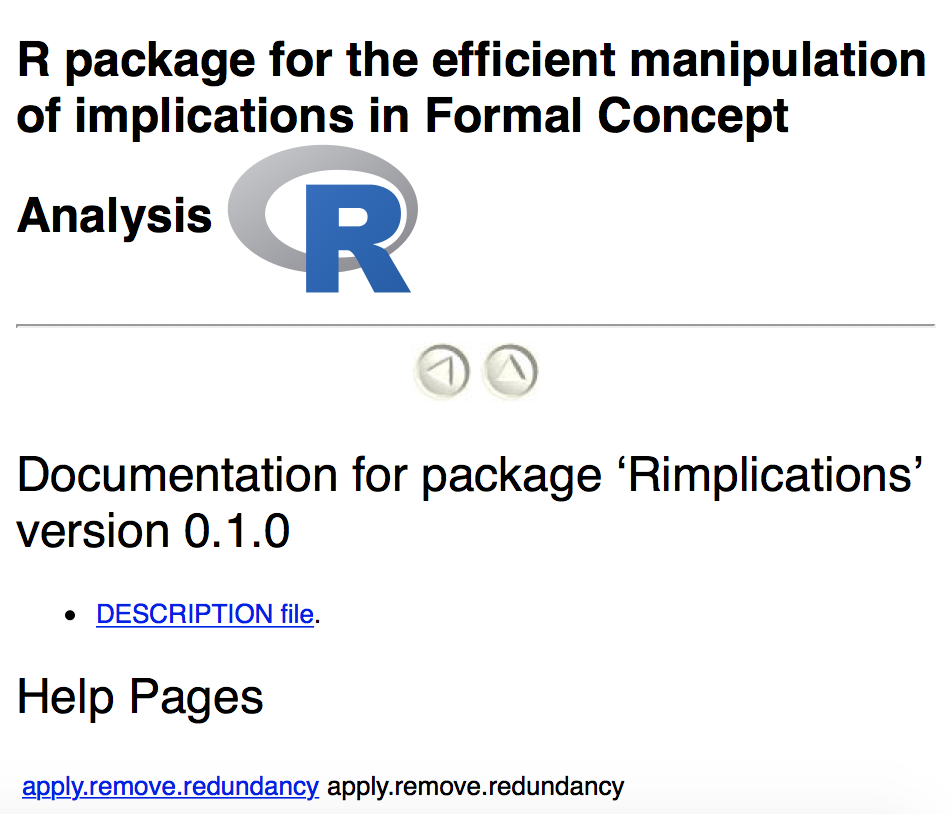
\includegraphics[scale=0.6]{docs2}
    \caption{Ejemplo Documentaci\'on 2}
    \label{fig:docs2}
\end{figure}

Aqu\'i se ve la documentaci\'on del algoritmo para la eliminaci\'on de redundancia:
\begin{figure}[H]
    \centering
    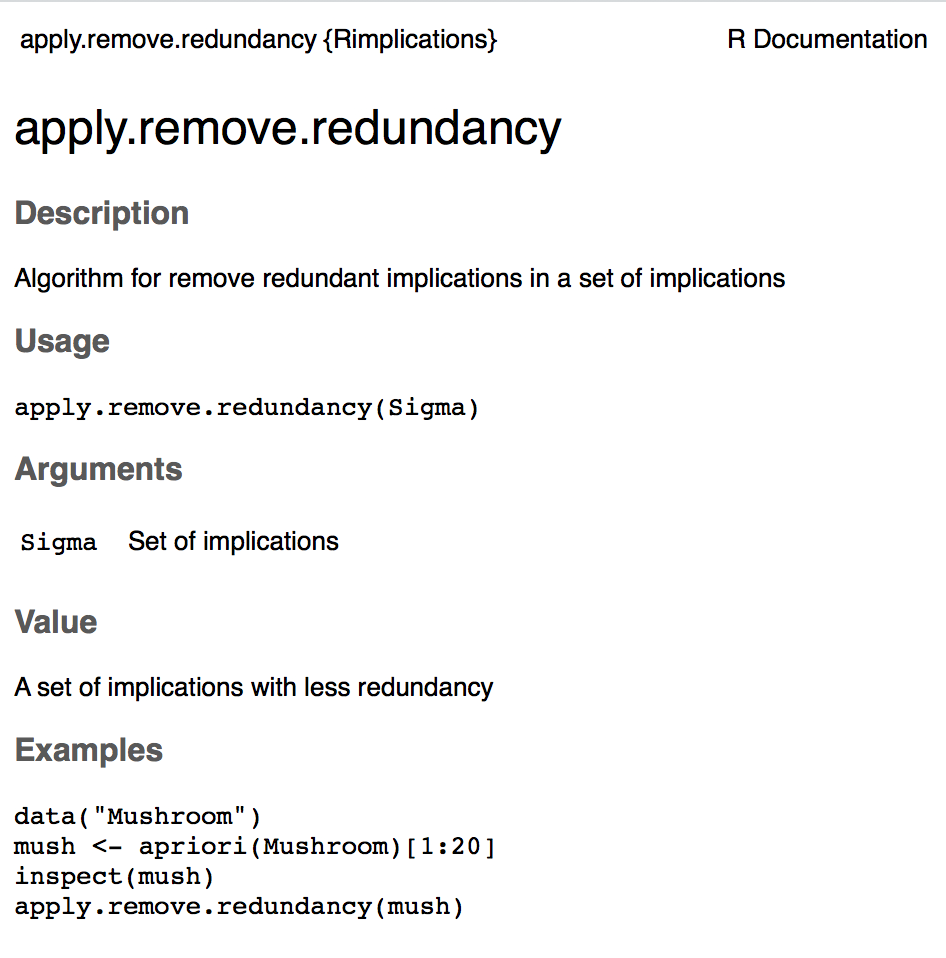
\includegraphics[scale=0.75]{docs3}
    \caption{Ejemplo Documentaci\'on 3}
    \label{fig:docs3}
\end{figure}
\newpage

\end{document}